
\documentclass[11pt]{article}

%\setlength\topmargin{-0.1in}
%\setlength\headheight{0in}
%\setlength\headsep{0in}
\setlength\textheight{8.5in}
\setlength\textwidth{6.5in}
\setlength\oddsidemargin{0in}
\setlength\evensidemargin{0in}
\setlength{\parindent}{0pt}
\usepackage{placeins}
%\usepackage{indentfirst}

\usepackage{amsmath}
\usepackage{graphicx}
\usepackage{listings}
\usepackage{rotating}
\usepackage{subcaption} 
\usepackage{booktabs}
\usepackage{tikz}
\usepackage{fancyhdr}
\usepackage{pdfpages}
\usepackage{hyperref}
\usepackage{longtable}
\usepackage[toc,page]{appendix}
%For The 2x2 Figure
\usepackage{subcaption}
\usepackage{mwe}
% To import matlab code
\usepackage{listings}
\usepackage{matlab-prettifier}
\usepackage[framed,numbered,autolinebreaks,useliterate]{mcode}
%Glossary
\usepackage[acronym,nonumberlist]{glossaries}
%\glsaddall %includes all acronymns
%Tables
\usepackage{booktabs}
\newcommand{\ra}[1]{\renewcommand{\arraystretch}{#1}}
%Nomenclature
\usepackage{nomencl}
\makenomenclature
\newif\iffirstglossary\firstglossarytrue
%% This removes the main title:
\renewcommand{\nomname}{}
%% this modifies item separation:
\setlength{\nomitemsep}{15pt}
%% this part defines the groups:
%----------------------------------------------
\usepackage{etoolbox}
\renewcommand\nomgroup[1]{%
  \item[\Large\bfseries
  \ifstrequal{#1}{N}{Nomenclature}{%
  \ifstrequal{#1}{A}{List of Abbreviations}{}}%
]\vspace{10pt}} % this is to add vertical space between the groups.
%----------------------------------------------



\pagestyle{fancy}
\usetikzlibrary{shapes,arrows}
\graphicspath{{Figures/}}
\newcommand{\tabitem}{~~\llap{\textbullet}~~}

\newcommand*{\MyIndent}{\hspace*{0.5cm}}%inerts tab in tables



 
\begin{document} 
\pagenumbering{gobble}

	\begin{titlepage}
	\thispagestyle{empty}
		\newcommand{\HRule}{\rule{\linewidth}{0.5mm}}	
		\center
		\LARGE 
		University of Bath\\
	 	Faculty of Engineering \& Design\\[1cm]	
		%textbf{\Large ME30313 Group Business & Design}\\
		\large
		Word count: 1584\\[0.5cm]
		{\large\today}\\[1cm]	
		\HRule\\[0.4cm]	
		{\LARGE \bfseries Systems Modelling \& Simulation Coursework 1}\\[0.3cm] 	
		\HRule\\[1cm]	
		\begin{minipage}{0.4\textwidth}
			\begin{flushleft}
				\large
				\textit{Supervisor}\\
				A. \textsc{Cookson}
			\end{flushleft}
		\end{minipage}
		~
		\begin{minipage}{0.4\textwidth}
			\begin{flushright}
				\large
				\textit{Assessor}\\
				
			\end{flushright}
		\end{minipage}\\[1.4cm]
		\large
		\textit{Author's Candidate Number}\\
		10838\\
		\vfill
		
\includegraphics[width=0.4\textwidth]{UOB_Logo.png}\\
		\vfill 
	\end{titlepage}

%%% ACRONYMS %%

%%END OF ACRONYMS %%%


\thispagestyle{empty}




\tableofcontents
\thispagestyle{empty}
\listoffigures


\nomenclature[A]{CAD}{Computer Aided Design}


%\printnomenclature


\clearpage
\pagenumbering{arabic}
%\setcounter{page}{1}
\section{Introduction}

This paper is based on solving the transient diffusion-reaction equation given by equation \ref{eq:MAIN}.


\begin{equation}\label{eq:MAIN}
\frac{\partial c}{\partial t}    = D\frac{\partial^2 c}{\partial x^2} + \lambda c + f
\end{equation}


\section{Part 1: Software Verification}

\subsection{Question 1a}
\subsubsection{Introduction}

A transient Diffusion-Reaction solver was developed and used to solve the specific transient equation give by equation \ref{eq:q1a}. This is the same equation as \label{eq:MAIN} with $\lambda = 0$ and $f = 0$. 

\begin{equation} \label{eq:q1a}
\frac{\partial c}{\partial t}    = \frac{\partial^2 c}{\partial x^2}
\end{equation}

The equation is subject to the following domain, boundary conditions and initial conditions.

\begin{equation*}
\begin{split}
x &= [0,1] \\
t &= [0,1] \\
c(x,0) &= 0 \\
c(0,t) &= 0 \\
c(1,t) &= 1
\end{split}
\end{equation*}

The analytical solution of equation \ref{eq:q1a} for the above conditions is given by equation \ref{eq:q1aAnal}.

\begin{equation} \label{eq:q1aAnal}
c(x,t) = x + \frac{2}{\pi} \sum_{n=1}^{\infty} \frac{(-1)^n}{n} e^{-n^2\pi^2t}\text{sin}(n\pi x)
\end{equation}



A Crank-Nicolson time stepping scheme was used with the recommended time step of $\delta t = .01$ and a 10 element mesh. The result produced using the finite element method is compared to the analytical solution for $ t = 0.01, \ 0.10, \ 0.20, \ 1$ as shown by Figure \ref{fig:q1a}. The FEM solver incorporates the option of quadratic basis functions and so this solution has been plotted in Figure \ref{fig:q1aquad} alongside the linear basis function solution shown in Figure \ref{fig:q1alin}. The difference between the quadratic and linear solutions is hardly noticeable in these plots and both provide a good approximation to the analytical solution. It is clear that the FEM solutions converge on the analytical solution as time increases with the plots indistinguishable at $t = 1$ where the steady state solution has been approached.

\begin{figure}[h!] 
        \centering
        \begin{subfigure}[b]{0.475\textwidth}
            \centering
            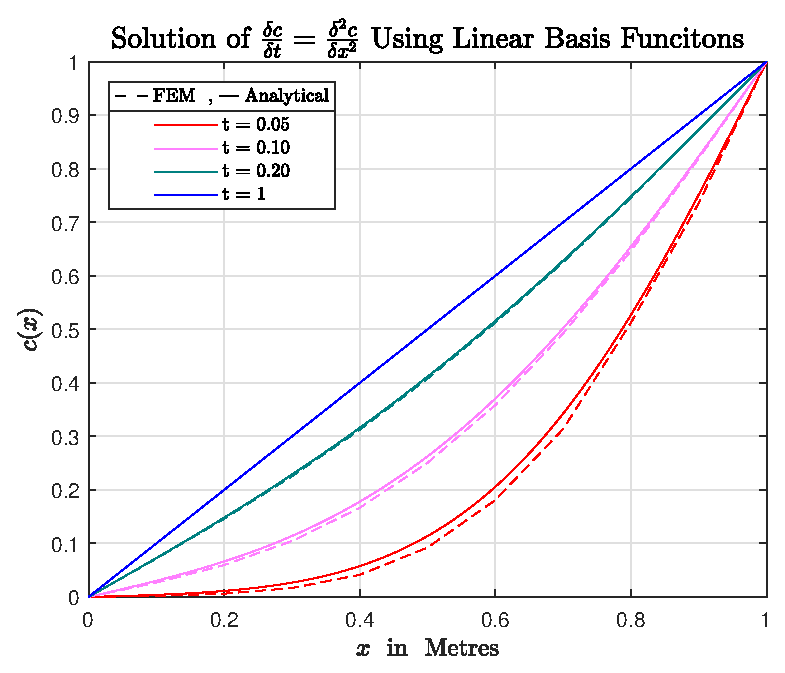
\includegraphics[width=\textwidth]{epsQ1a}
            \caption[]%
            {{\small Linear Basis Function Solution }}    
            \label{fig:q1alin}
        \end{subfigure}
        \hfill
        \begin{subfigure}[b]{0.475\textwidth}  
            \centering 
            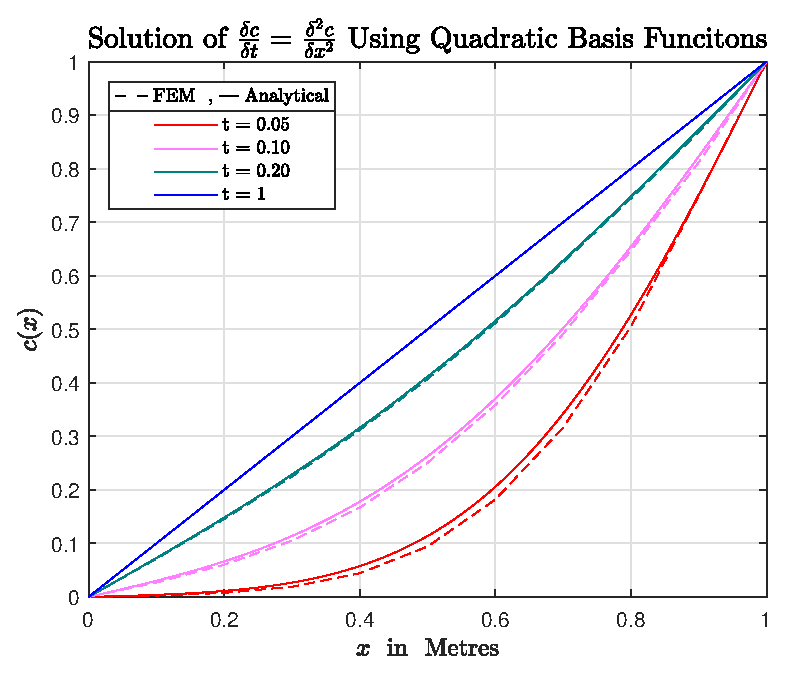
\includegraphics[width=\textwidth]{epsQ1aQuad}
            \caption[]%
            {{\small Quadratic Basis Function Solution}}    
            \label{fig:q1aquad}
        \end{subfigure}
        \caption[ The Effect of Mesh Size on Temperature Resolution ]
        {\small Comparison of FEM with Crank-Nicolson Time Stepping and Analytical Results.} 
        \label{fig:q1a}
\end{figure}


\subsection{Investigation of Time Stepping Schemes}

The times stepping schemes used were Backward Euler and Crank-Nicolson. The results at $x = 0.8m$ for over the time range have been plotted both time stepping schemes at time steps of $\Delta t = 0.1s$ and $\Delta t = 0.025s$ in Figures \ref{fig:q1b05} and \ref{fig:q1b025} respectively. With a time step of $\Delta t = 0.1s$  the Crank-Nicolson scheme is showing oscillatory solution whereas the Backward Euler scheme does not oscillate. The oscillatory response of the Crank-Nicolson reduces with time and even at the large time step is more accurate over the time domain than the Backward Euler scheme. As the time step is reduced to $\Delta t = 0.02s$ the oscillation of the Crank-Nicolson scheme is much reduced as is again clearly more accurate that the Backward Euler scheme.


\begin{figure}[ht] 
        \centering
        \begin{subfigure}[b]{0.475\textwidth}
            \centering
            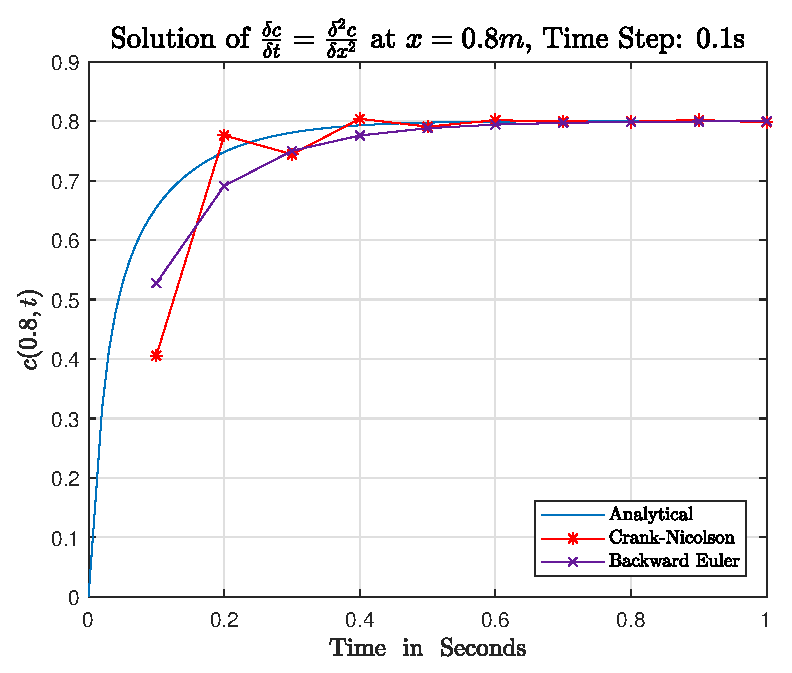
\includegraphics[width=\textwidth]{epsQ1bdt05}
            \caption[]%
            {{\small Time Step of 0.1s }}    
            \label{fig:q1b10}
        \end{subfigure}
        \hfill
        \begin{subfigure}[b]{0.475\textwidth}  
            \centering 
            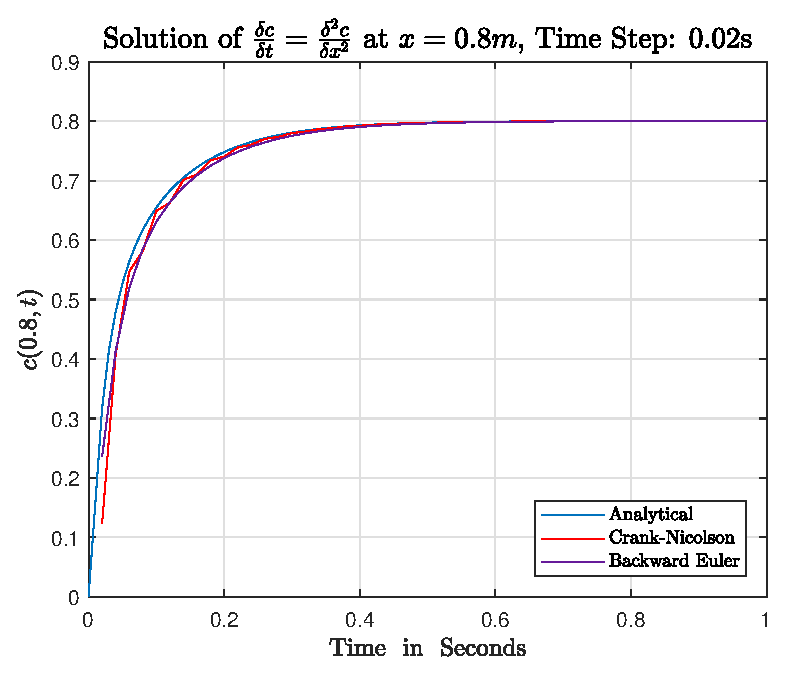
\includegraphics[width=\textwidth]{epsQ1bdt025}
            \caption[]%
            {{\small Time Step of 0.02s}}    
            \label{fig:q1b025}
        \end{subfigure}
        \caption[ The Effect of Mesh Size on Temperature Resolution ]
        {\small Comparison of Crank-Nicolson and Backward Euler Time Stepping Schemes, $dx = 0.1$} 
        \label{fig:q1b025}
\end{figure}

\FloatBarrier
\subsection{Investigating the L2 Norm}

The L2 norm is the error of the FEM solution compared to the analytical solution. As the $L_2$ Norm is investigating the error in the  spatial domain the time step had to be very small to make the time error insignificant. As a result only low resolution meshes could be tested to keep computing time reasonable. Equation \ref{eq:l2norm1} shows how the exact solution $CE(x)$ is approximated by the FEM solution $C(x)$ with an additional higher order terms truncated. For linear basis functions the lowest order truncated term, n,  is $n = 2$, and similarly for quadratic basis functions $n = 3$.

\begin{equation} \label{eq:l2norm1}
CE(x) = C(x) + O(h^n)
\end{equation}

The error $E(x)$ is $CE(x) - C(x)$ and by rewriting the higher $O(h^n)$ as $Gh^n$, where $G$ is a constant, equation \ref{eq:l2norm1} can be written as equation \ref{eq:l2normgrad}. It can be seen that as the error converges with increasing mesh resolution the gradient of the a logarithmic plot of these should be $n$. 


\begin{equation} \label{eq:l2normgrad}
log(E(x)) = log(G) + n*log(h)
\end{equation}

The $L_2$ norm was calculated for mesh sizes of 5 to 12 elements and plotted as shown in Figures \ref{fig:q1l2o1} and \ref{fig:q1l2o2} for linear and quadratic basis functions respectively. The gradients were computed to be -1.97 and -2.88 for linear and quadratic plots respectively. This shows that the $L_2$ norm is converging as the gradients match the expected $n$ values of the truncated terms. 


\begin{figure}[ht] 
        \centering
        \begin{subfigure}[b]{0.475\textwidth}
            \centering
            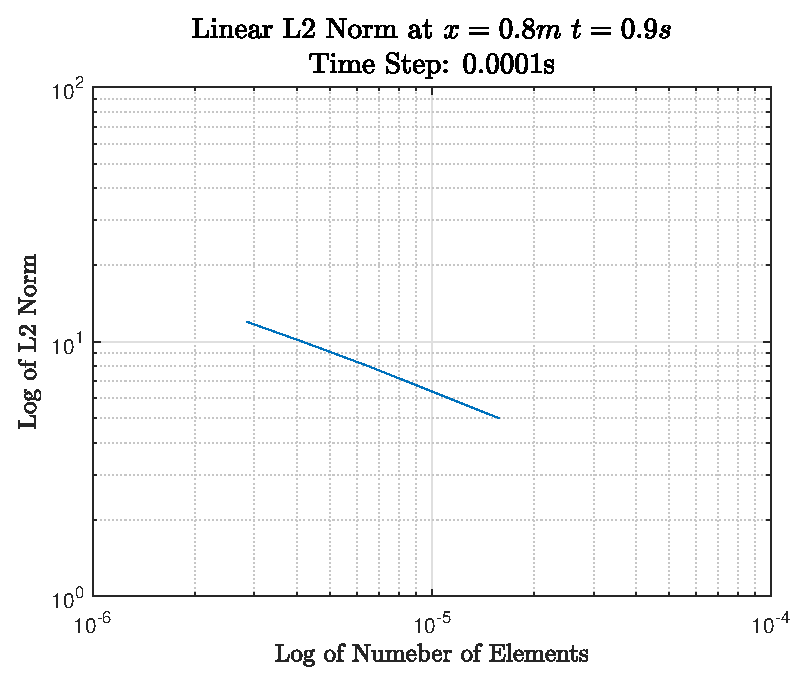
\includegraphics[width=\textwidth]{epsQ1L2O1}
            \caption[]%
            {{\small Gradient = -1.97 }}    
            \label{fig:q1l2o1}
        \end{subfigure}
        \hfill
        \begin{subfigure}[b]{0.475\textwidth}  
            \centering 
            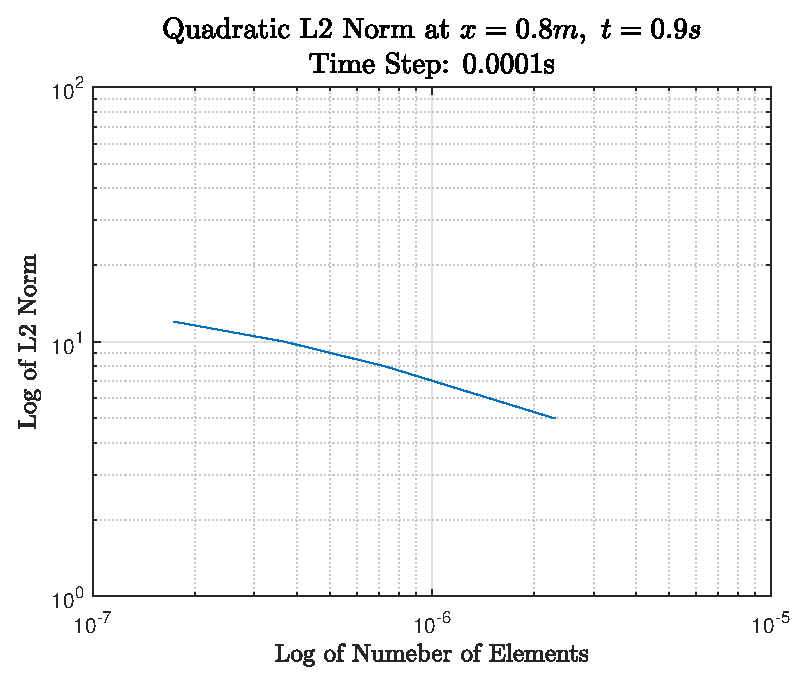
\includegraphics[width=\textwidth]{epsQ1L2O2}
            \caption[]%
            {{\small Gradient = -2.88}}    
            \label{fig:q1l2o2}
        \end{subfigure}
        \caption[ ]
        {\small Comparison of Error Conversion for Linear and Quadratic Basis Functions.} 
        \label{fig:q1bl2grad}
\end{figure}
\pagebreak


\section{Part 2: Modeling and Simulation Results}

\subsection{Question 1}

The code developed in Part 1 was used to model heat transfer through skin. The skin is split into layers and the heat tranfer through the first three layers was investigated. The spatial domain, $x$, is defined by Figure \ref{fig:skinlayers} where the boundaries are defined as:
\begin{equation*}
 B = 0.01 \ , \ \ D = 0.005 \ , \ \ E  =  0.00166667.
\end{equation*}

\begin{figure}[!h]  %nrcVrc Figure
	\centering
	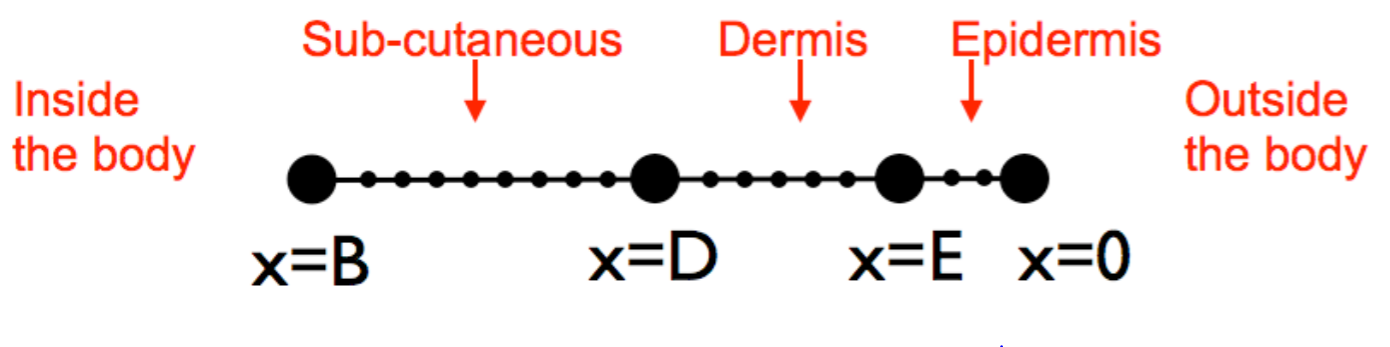
\includegraphics[width=.75\textwidth]{SkinStructure.png}
    \caption{Layout of Skin Layers and the $x$ Domain. XXX REF}\label{fig:skinlayers}
\end{figure}

The material properties are not consistent between layers and are defined in Table \ref{table:defparams}.
\FloatBarrier
\begin{table}[!h]
\centering %Set parameters table
\ra{1.3}
\begin{tabular}{@{}cccc@{}}\toprule
 \textbf{Parameter}  & \textbf{Epidermis} &  \textbf{Dermis} & \textbf{Sub-cutaneous} \\
\midrule
$ k$ & 25  &  40  & 20 \\
$G$ & 0  & 0.0375  & 0.0375 \\
$\rho$ & 1200  &  1200  &  1200 \\
$c$ & 3300 & 3300  & 3300 \\
$\rho_b$ & -  & 1060  & 1060 \\
$c_b$ & -  & 3770  &  3770\\
$T_b$  & - & 310.15  &  310.15  \\
\bottomrule
\end{tabular}
\caption{Material Properties of Skin at Each Layer.}
\label{table:defparams}
\end{table}
\FloatBarrier

The governing equation of heat transfer over the $x$ domain is given by equation \ref{eq:goveqn} where parameters are not consistent between layers and are defined in Table \ref{table:defparams}.

\begin{equation} \label{eq:goveqn}
\frac{\partial T}{\partial t}    = \bigg(\frac{k}{\rho c} \bigg)\frac{\partial^2 T}{\partial x^2} - \bigg(\frac{G \rho_b c_b}{\rho c}\bigg)T + \bigg(\frac{G \rho_b c_b}{\rho c}\bigg)T_b
\end{equation}

\begin{figure}[!h]  %nrcVrc Figure
	\centering
	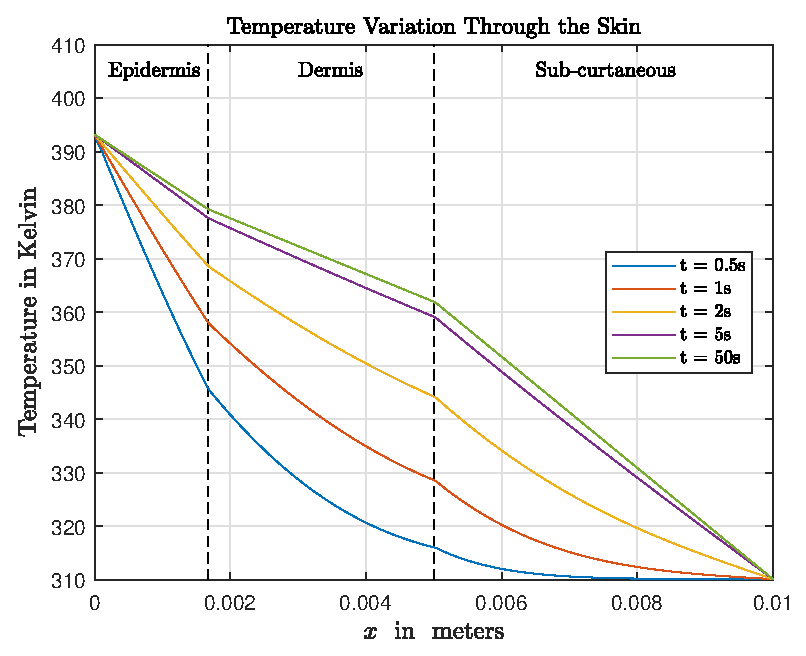
\includegraphics[width=.75\textwidth]{epsQ21TempXT}
    \caption{Temperature Profiles as Time Increases. }\label{fig:q21profs}
\end{figure}


\subsection{Question 2}


The function EvalGamma.m shown in Appendix XXX, was created to return the value of $\Gamma$ for a given boundary condition temperature at $x = 0$. The required value of $\Gamma$ to avoid second degree burns is $\Gamma = 1$. From Part 2 Question 1 it was known that a boundary condition of $T(0, t) = 393.15K$ produced a values of Gamma many orders of magnitude greater than $\Gamma = 1$. Furthermore as the temperature which burning occurs is $T_{burn} = 317.15$ it follows that a boundary condition of $T(0, t) = 393.15K$ will produce the result  $\Gamma < 1$. \\

\begin{table}[!h]
\centering %Set parameters table
\ra{1.3}
\begin{tabular}{@{}ccccl@{}}\toprule
 Iteration  & $T_{high}$ (K) & $T_{low}$ (K) &  $T_{av}$ (K) & $\Gamma (T_{av}) $ \\
\midrule
1 \   & 394 & 316  &  355  &  2.05e+29\\
2 \   & 355 & 316  &  335.5  & 4.75e+09 \\
3 \   & 335.5 & 316  &  325.75  &  1.13e-05 \\
4 \   & 335.5 & 325.75  & 330.63  & 825 \\
5 \   & 330.63 & 325.75  &  328.19  & 0.138 \\
6 \   & 330.63 & 328.19  & 329.41  &  11.58\\
7 \   & 329.41 & 328.19  &  328.80  & 1.2892  \\
8 \   & \textbf{328.80} & 328.19  &  \textbf{328.49}  & 0.4233  \\
\midrule
Result & 328.8 & 328.5 & 328.6 & 0.74\\
\bottomrule
\end{tabular}
\caption{Result of FindBC.m XXX. at Each Iteration.}
\label{table:findbc}
\end{table}

A script was made to calculate the value $T(0,t)$ to within 0.5K which would produce a result of $\Gamma = 1$ called XXX.m shown in Appendix XXX. The process followed to find the boundary condition is described by the flow chart in Figure \ref{fig:BCflowchart}. The initial high and low temperature bounds were set at $T(0, t) = 394K$ and $T(0, t) = 316K$ to respectively to give result for $\Gamma$ above and below the target value of $\Gamma = 1$ as previously explained. The process took 8 iterations to find the temperature range of 0.5K which contained the boundary condition, $T(0, t) =T$, which results in $\Gamma = 1$. The range found by was $T(0,t) = 328.5K \ \text{to} \ 328.8K$. \\
 It was difficult to design a more efficient algorithm such as the shooting method to determine the boundary condition due to the extreme non-linearity between $\Gamma$ and $T(0,t)$. The result at each iteration of FindBC.m XXX is shown in Table \ref{table:findbc} and gives insight into how the algorithm arrived at the solution of $T(0, t) =T$. The temperature variation with time at the Epidermis boundary has been plotted at selected iterations in Figure \ref{fig:q22profs}. The boundary condition for each interval in Figure \ref{fig:q22profs} is given by the $T_{av}$ for the corresponding iteration in Table \ref{table:findbc}.



\begin{figure}[ht]  %nrcVrc Figure
	\centering
	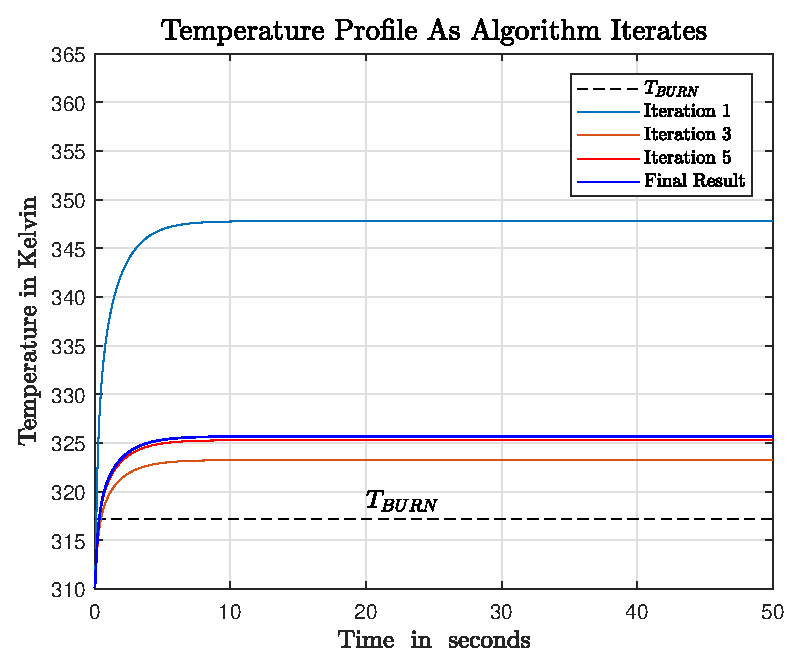
\includegraphics[width=.75\textwidth]{epsQ22BCTempProfs}
    \caption{Temperature Profiles As Algorithm Converges on $\Gamma = 1$.}\label{fig:q22profs}
\end{figure}

\begin{figure}[ht]  %nrcVrc Figure
	\centering
	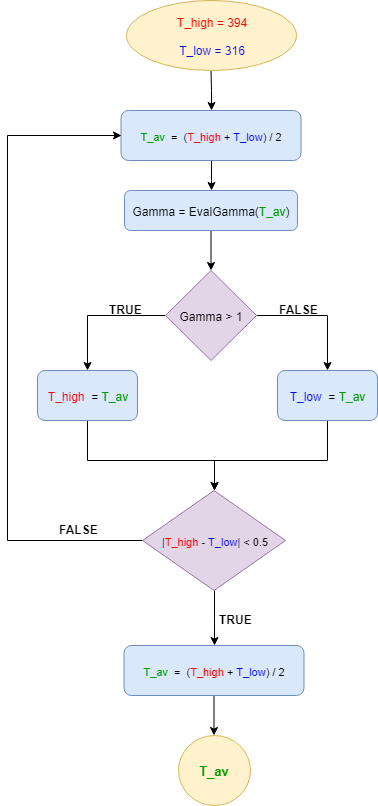
\includegraphics[width=.6\textwidth]{FindBCFlow.png}
    \caption{Flow Chart Showing The Process Followed by The XXX BCFinder.m Script}\label{fig:BCflowchart}
\end{figure}

%%\\\\\\\\\\\\\\\\\\\\\\\\\\\\\\\\\      APPENDICIES         \\\\\\\\\\\\\\\\\\\\\\\\\\\\\\\\\\\\\\\\\\\\\\\\\\\\\\\\\\\\\%%%%%%%%
\FloatBarrier
\begin{appendices}

\section{Flow Chart of FEM Solver}

\begin{figure}[ht]  %nrcVrc Figure
	\centering
	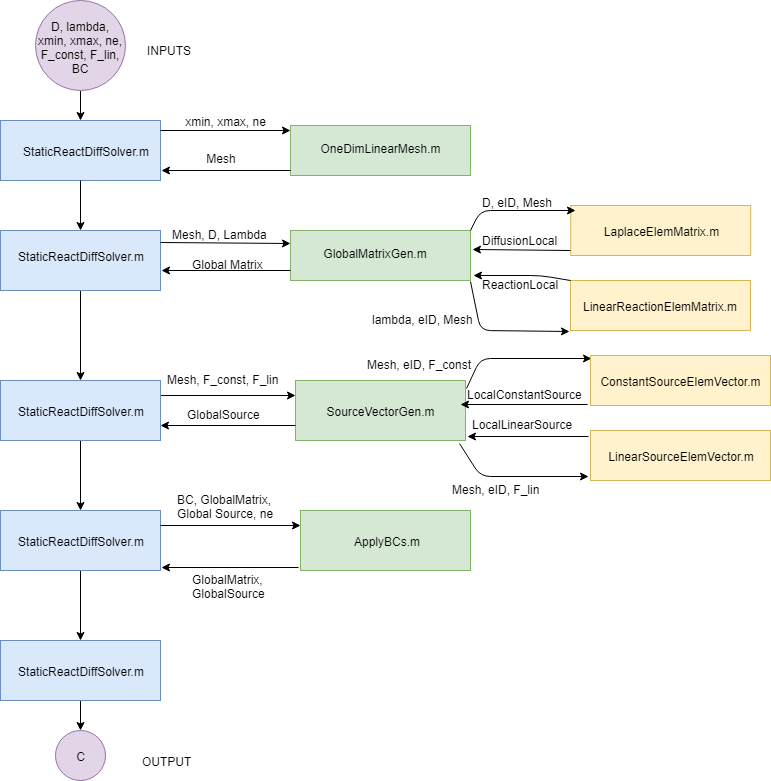
\includegraphics[width=1\textwidth]{FLOW.png}
    \caption{Flow Chart Showing The Process Followed by The FEM solver StaticReactDiffSolver.m}\label{fig:flowchart}
\end{figure}
\clearpage
%%AAAAAAAAAAAAAAAAAAAAAAAAAA%%%%%%%
\section{Laplace Element Matrix Code}\label{ap:LaplaceElem}


J = msh.elem(eID).J;  %Get Jacobi for the element
\begin{lstlisting}
function [SqMatrix] = LaplaceElemMatrix(D, eID, msh)

SqMatrix = [0.5, -0.5; ...
            -0.5, 0.5];

%% Multiply  by (1/J) and D to get solution for the particular element
SqMatrix = (1/J) * D * SqMatrix;   %Local element matrix for element eID
end
\end{lstlisting}
\pagebreak






\end{appendices}





\end{document}

